\documentclass[11pt]{article}
\usepackage[margin=1in]{geometry}
\usepackage{lmodern}
\usepackage{microtype}
\usepackage{setspace}
\usepackage{xcolor}
\usepackage{hyperref}
\usepackage{pdfpages}
\usepackage{booktabs}
\hypersetup{colorlinks=true,linkcolor=blue!50!black,urlcolor=blue!60!black}
\pagestyle{empty}
\begin{document}
\begin{center}
\vspace*{1.0in}
{\Huge\bfseries All Gods Must Die\\[0.25em]}
{\LARGE Adversarially Verified Transformation\\[1.25em]}
{\Large Successor Release v1.1\\[0.5em]}
{\large Incorporating Amendment I: Task Completion Verification\\[2em]}
{\large Axl Ibiza, MBA\\[0.35em]}
{\normalsize August 21, 2026}
\end{center}

\vfill

\begin{quote}
\textbf{Revision law.} This release does not silently rewrite the August 2026 publication. It preserves the original 68-page v1.0 artifact byte-for-byte and appends a separately sourced, separately digestible amendment. The composed PDF is the canonical successor release for the expanded doctrine.
\end{quote}

\vspace{1em}

\begin{tabular}{@{}p{0.27\textwidth}p{0.65\textwidth}@{}}
\toprule
\textbf{Component} & \textbf{Identity and role} \\
\midrule
Original publication & \texttt{all-gods-must-die-adversarially-verified-transformation.pdf}; SHA-256 \texttt{76310ddf1d1f56745a105ca9ff32b72ea809ebdbb89fe1a385196e3050a1e056}. Immutable v1.0 body. \\
Amendment I & \texttt{task-completion-verification-amendment.pdf}. Adds exact-object, state-typed completion doctrine and the sixth law. \\
Composed release & This wrapper plus the two PDFs above. The release manifest carries the final component digests and typed lineage. \\
\bottomrule
\end{tabular}

\vfill

\begin{center}
\emph{No task is complete until the requested state exists at the authoritative target and is verified on the exact object.}
\end{center}

\clearpage
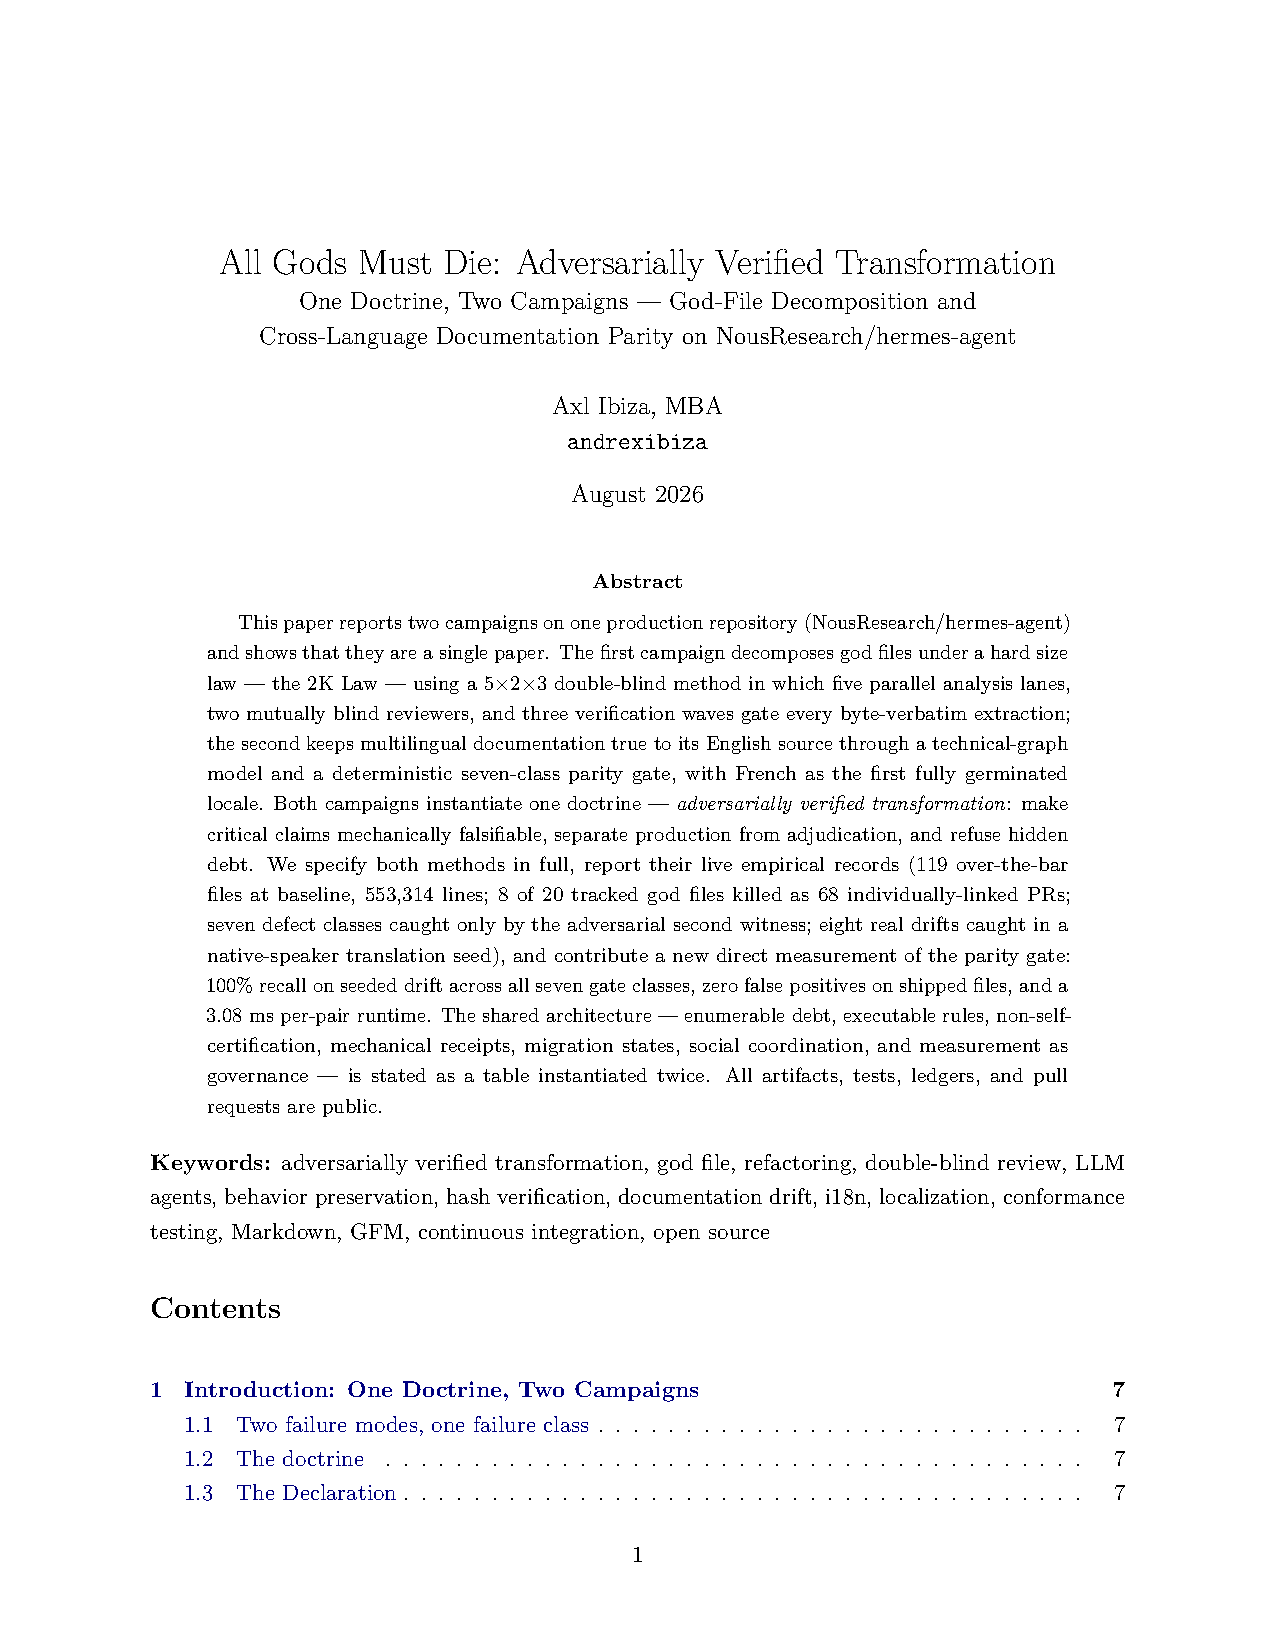
\includepdf[pages=-,pagecommand={}]{all-gods-must-die-adversarially-verified-transformation.pdf}
\includepdf[pages=-,pagecommand={}]{task-completion-verification-amendment.pdf}
\end{document}
